\section{Editor de modelos gráfico generado a partir de los proyectos edit,editor}

Eclipse EMF permite generar objetos a partir de los modelos creados en \gls{ecore} de forma gráfica. 

Esto puede ser útil, ya que no tiene porque ser necesaria la creación de un \gls{dsl} como veremos en la próxima sección. 

Con el propio editor creado, alguien con los conocimientos suficientes podría generar un modelo ejecutable por un entorno EMF, siempre que contenemos con el \textit{runtime} necesario para leer este modelo.

El editor por defecto utilizará los iconos standard para los elementos de nuestro modelo. Esto si es modificado nos permite que el usuario de forma rápida sea capaz de situarse en el elemento necesario. Por ejemplo, podríamos asociar el icono de un diodo \gls{led} a los elementos salida \gls{gpio}, o un icono de un botón, a un elemento evento pulsador.


\subsection{Ejecución de EMF en modo runtime}

Para realizar esta tarea, a partir de nuestro proyecto \gls{ecore} principal y una vez generados los proyectos necesarios edit y editor, ejecutaremos \gls{emf} en modo \gls{runtime}, tal como vemos en la figura \ref{fig:runtime_emf_paso1}. Una vez seleccionado, seleccionaremos \textit{Run as eclipse runtime}  (Ver figura \ref{fig:runtime_emf_paso2}).

\begin{figure}
	\centering
    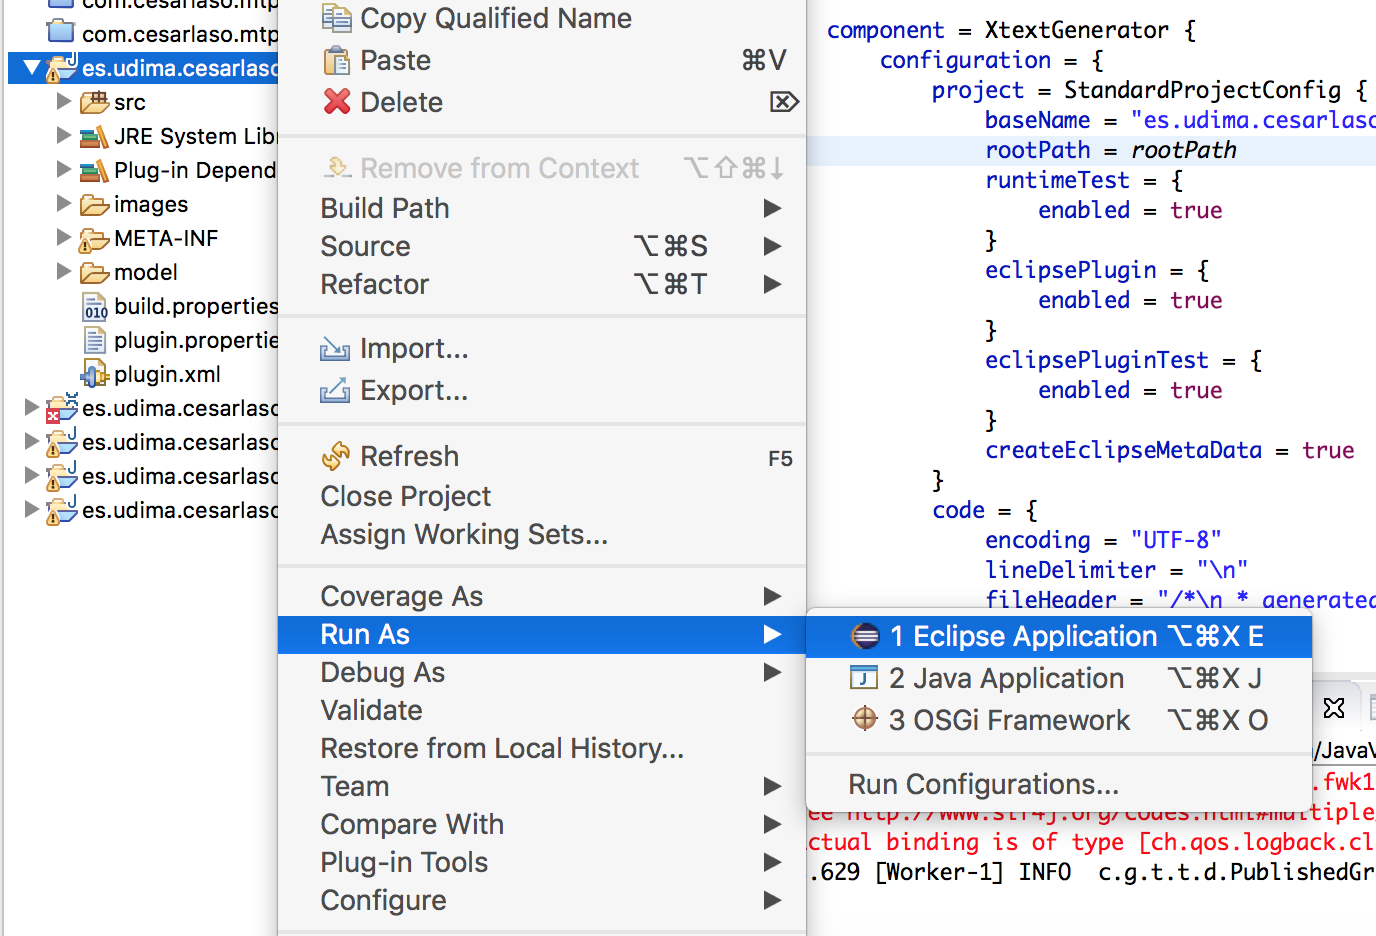
\includegraphics[scale=0.4]{images/emf_capturas/runtime_emf_paso1}
    \sourcepropia{}
    \caption{Ejecutar EMF en modo runtime desde proyecto existente - Paso 1}
    \label{fig:runtime_emf_paso1}
\end{figure}

\begin{figure}
	\centering
    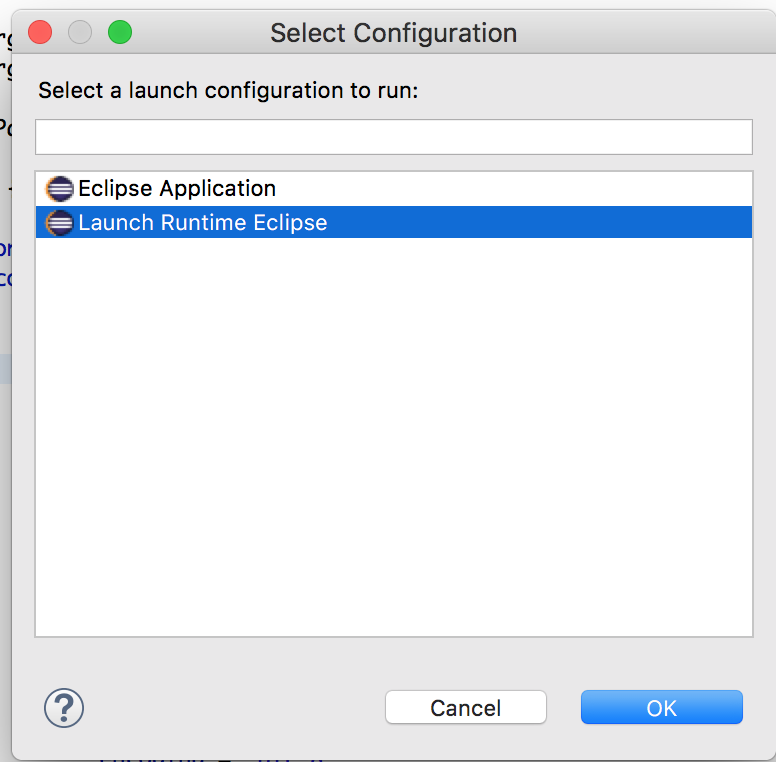
\includegraphics[scale=0.4]{images/emf_capturas/runtime_emf_paso2}
    \sourcepropia{}
    \caption{Ejecutar EMF en modo runtime desde proyecto existente - Paso 2}
    \label{fig:runtime_emf_paso2}
\end{figure}


Una vez tenemos lanzado \gls{emf} en modo \gls{runtime}, crearemos un nuevo proyecto vacío, no importa el tipo de proyecto a utilizar, podemos por ejemplo utilizar un proyecto base de java.

Una vez creado, vamos a utilizar los \texit{wizard} generados automáticamente por los generadores de código anteriormente nombrados, para ello crearemos un nuevo archivo de tipo \textit{EMF model wizard} seleccionando nuestro tipo de modelo \textit{IotProyect}, tal como vemos en la figura \ref{fig:runtime_editor_wizard}.

\begin{figure}
	\centering
    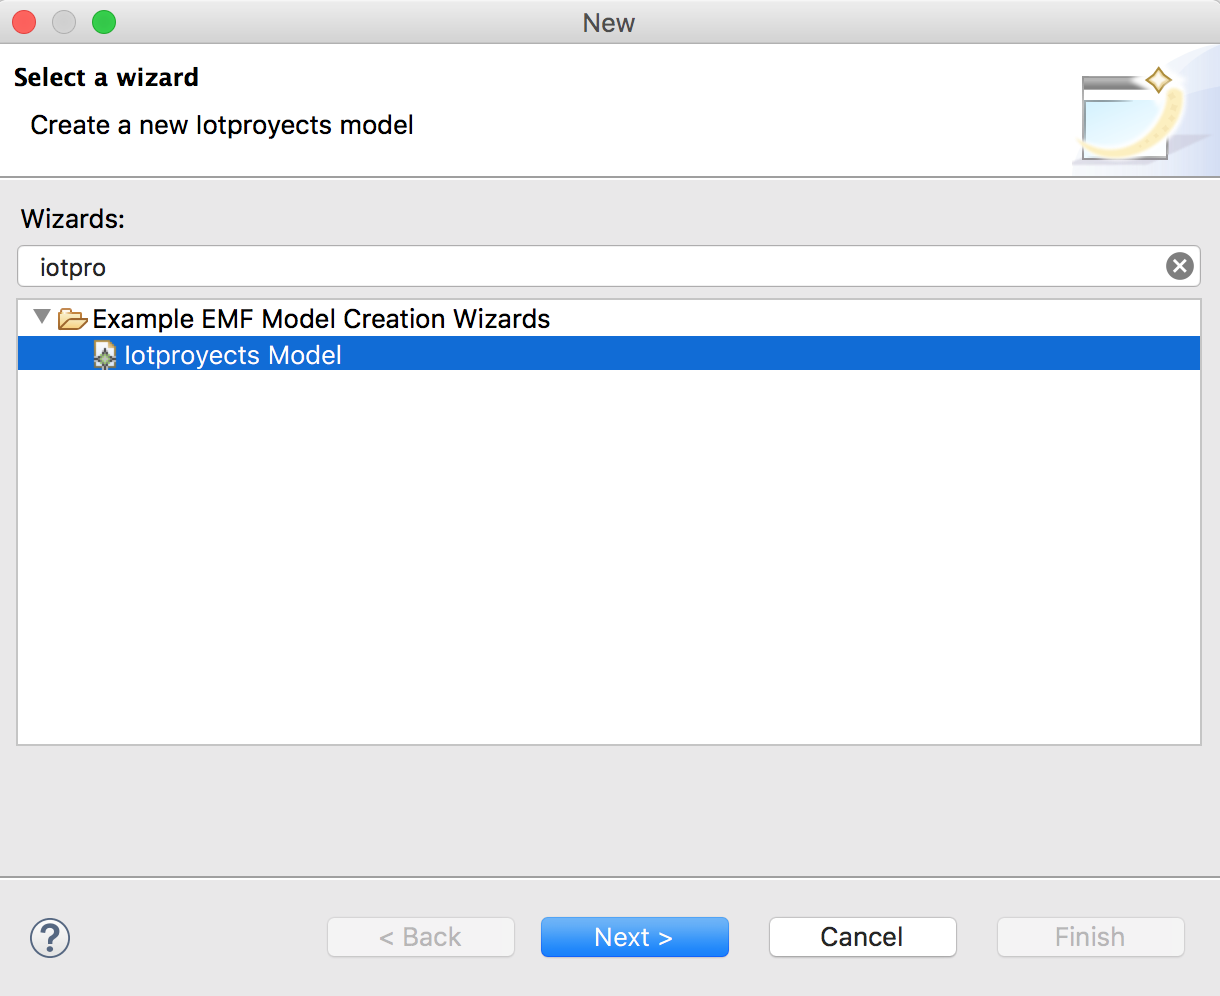
\includegraphics[scale=0.4]{images/emf_capturas/runtime_editor_wizard}
    \sourcepropia{}
    \caption{EMF Wizard - Creación de un objeto a partir de un modelo de forma gráfica}
    \label{fig:runtime_editor_wizard}
\end{figure}

Este editor nos permite crear objetos del modelo en forma de árbol, permitiéndonos desde el propio entorno gráfico modelar un programa a partir del meta-modelo \gls{ecore}, tal como vemos en la figura \ref{fig:runtime_editor_modelo1}.

El editor nos autocompletará (ver figura \ref{fig:runtime_editor_modelo2}) con los elementos permitidos en cada sección del metamodelo.

\begin{figure}
	\centering
    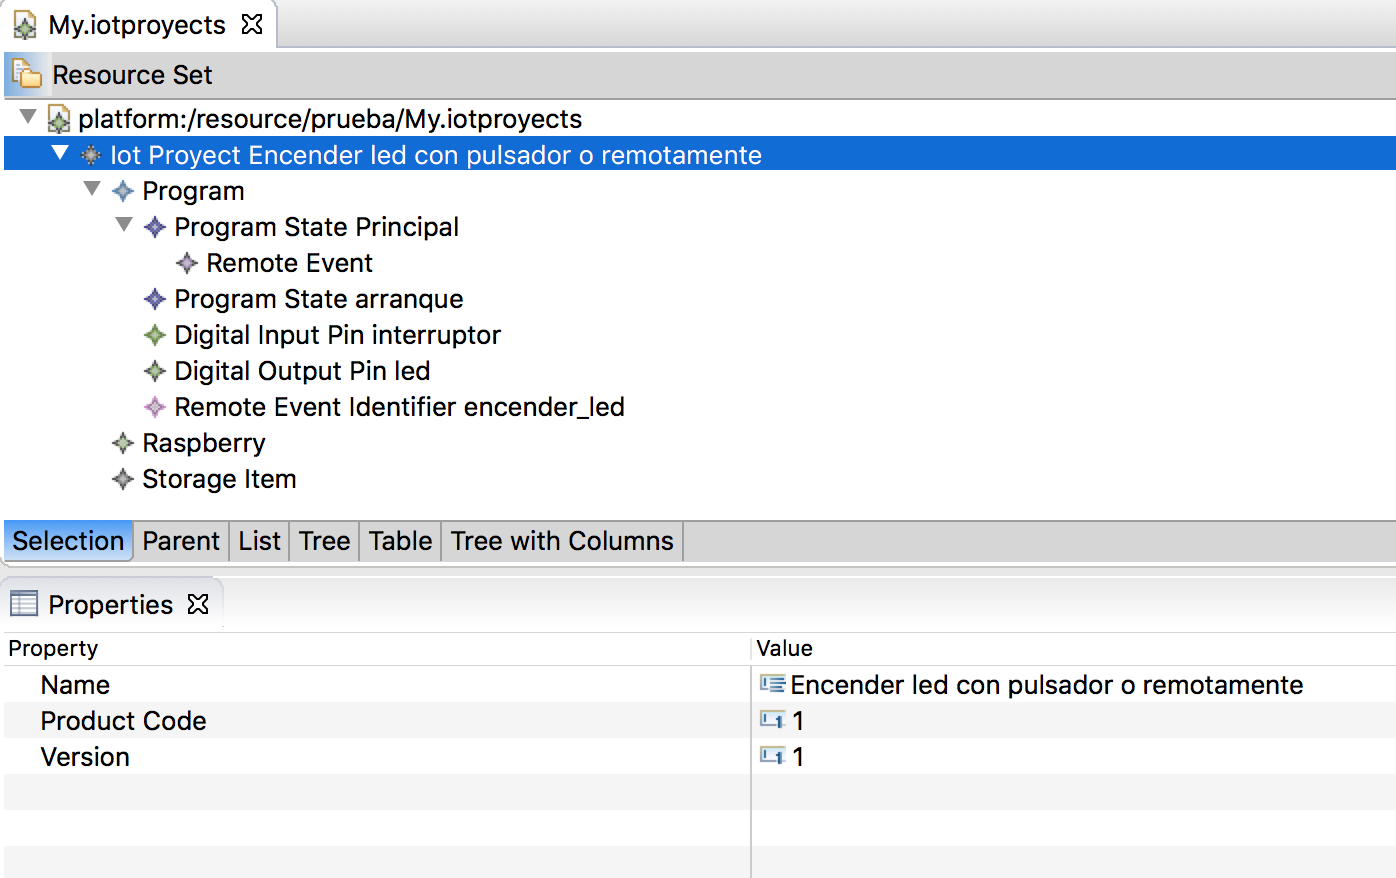
\includegraphics[scale=0.4]{images/emf_capturas/runtime_editor_modelo1}
    \sourcepropia{}
    \caption{Editor gráfico del modelo a partir de metamodelo ecore}
    \label{fig:runtime_editor_modelo1}
\end{figure}

\begin{figure}
	\centering
    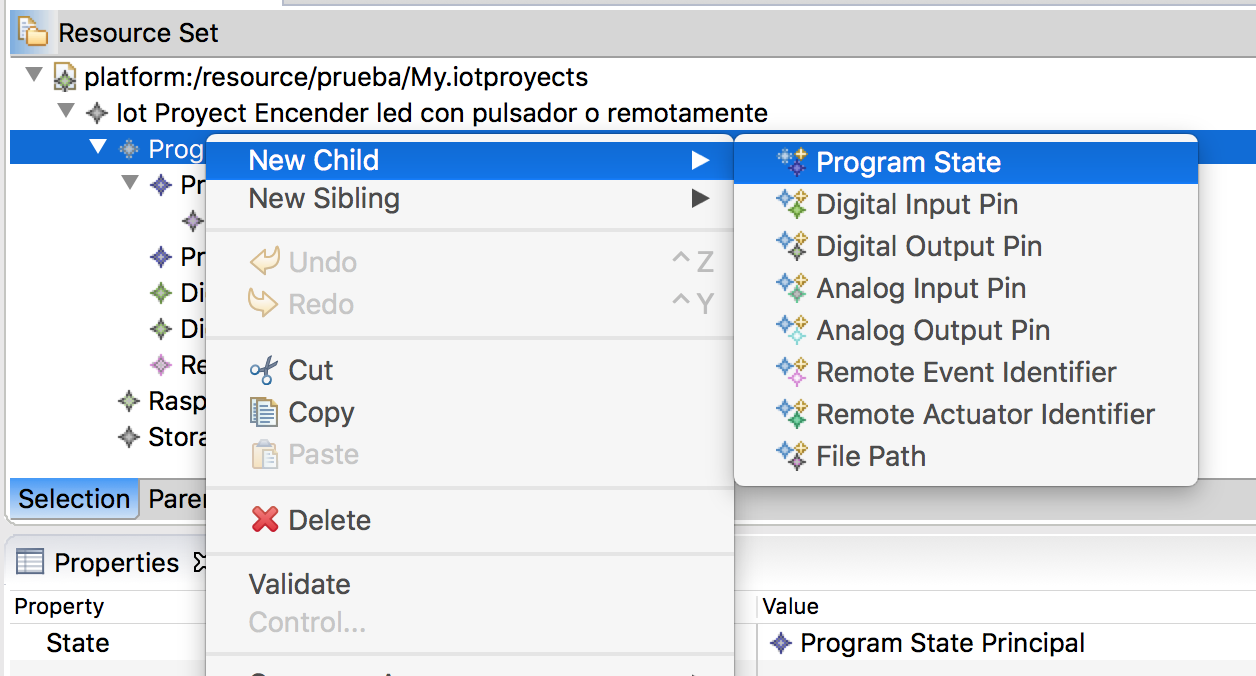
\includegraphics[scale=0.4]{images/emf_capturas/runtime_editor_modelo2}
    \sourcepropia{}
    \caption{El editor gráfico nos ayuda en la selección de subelementos}
    \label{fig:runtime_editor_modelo2}
\end{figure}


\subsection{GMP Graphical model proyect}

Mediante \cite{gmp} podemos ampliar el editor generado anteriormente y darle un aspecto totalmente personalizado para nuestro dominio de trabajo.
\gls{gmp} proporciona un kit completo de desarrollo, incluyendo el editor gráfico \gls{gmf}.

Este tipo de editor requiere bastante esfuerzo adicional y queda fuera del alcance del proyecto, pero su mención es totalmente necesaria ya que nos permite crear editor gráficos basados en el editor \gls{emf} y totalmente en este caso adaptados al dominio.

En la figura \ref{fig:gmf_ejemplo} se muestra un ejemplo. Este ejemplo podemos verlo completo en el tutorial de \gls{gmf} \cite{gmf_tutorial}.

\begin{figure}
	\centering
    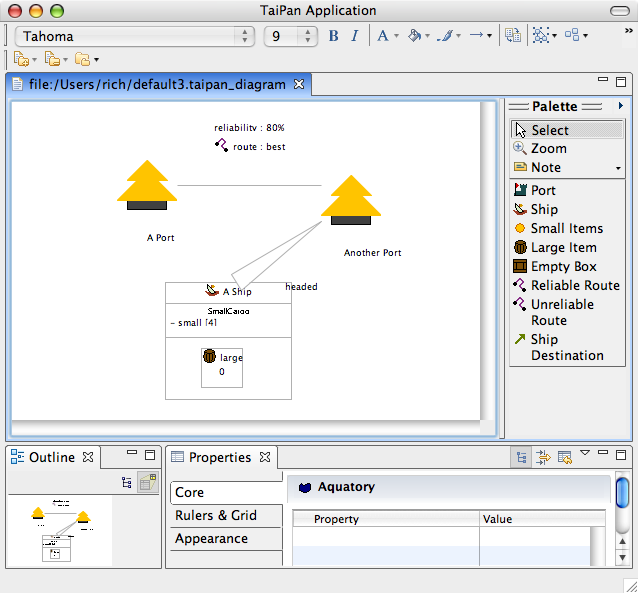
\includegraphics[scale=0.4]{images/emf_capturas/gmf_ejemplo}
    \source{Web GMF \cite{gmf_tutorial}}
    \caption{GMF permite personalizar el editor de objetos modelo a un nivel mayor.}
    \label{fig:gmf_ejemplo}
\end{figure}






